\documentclass{article}

% Language setting
% Replace `english' with e.g. `spanish' to change the document language
\usepackage[english]{babel}

% Set page size and margins
% Replace `letterpaper' with`a4paper' for UK/EU standard size
\usepackage[letterpaper,top=2cm,bottom=2cm,left=3cm,right=3cm,marginparwidth=1.75cm]{geometry}

% Useful packageshttps://www.overleaf.com/project/617db8234c85bd8404625de7
\usepackage{amsmath}
\usepackage{graphicx}
\usepackage{amsthm}
\usepackage{amssymb}
\usepackage[colorlinks=true, allcolors=blue]{hyperref}
\usepackage[dvipsnames]{xcolor}
\newtheorem{theorem}{Theorem}[section]
\newtheorem{corollary}{Corollary}[theorem]
\newtheorem{lemma}[theorem]{Lemma}
\usepackage{float}

\theoremstyle{definition}
\newtheorem{definition}{Definition}[section]

\theoremstyle{remark}
\newtheorem*{remark}{\textbf{Remark}}

\theoremstyle{example}
\newtheorem{example}{\textbf{Example}}[section]

\title{Proof of the Existence and Uniqueness Theorem\\
\begin{large} 
  MST-311 Final Project
\end{large}}
\author{Ruiqi (Rickey) Huang, Zhanyang Sun, Lyle Huang}

\newcommand{\qedwhite}{\hfill \ensuremath{\Box}}

\begin{document}
\maketitle

\begin{abstract}
    The goal of this project is to prove the Existence and Uniqueness Theorem for ordinary differential equations in the form of $\tfrac{\,dy}{\,dt} = f(t,y), y(0) = y_0$. The theorem will be proved in $\mathbb{R}$ first using the Banach Fixed Point Theorem. We will introduce the method of successive substitution, which is also called Picard's Iteration in the operator case, to approximate the unique solution of the given ordinary differential equation. After this, the Existence and Uniqueness Theorem will be stated and proved again in a general metric space defined as $(X,d)$ with a norm induced metric $d$ by applying the Contraction Mapping Theorem.
\end{abstract}

\section{Introduction}

\paragraph{  }

Even though we are equipped with many methods of solving ordinary differential equations in some particular forms, like linear, exact, separable, substitution, and transformation, the ordinary differential equations that we are able to solve and get explicit formula are only a small proportion of all of them. This makes the Existence and Uniqueness Theorem important for us since it shows whether an ordinary equation has a solution on a certain interval. 

\paragraph{  }

The Existence and Uniqueness Theorem could be applied to different types of ordinary differential equations. In this paper, we focus on the ordinary differential equations in the form of $\tfrac{\,dy}{\,dt} = f(t,y),\; y(0) = y_0$. The theorem in $\mathbb{R}$ is stated as the following:

%\begin{definition}[\textbf{Lipschitz Function}]\label{def:Lip}
 %   A function $f(x)$ is a \textbf{Lipschitz Function} if and only if 
 %   \begin{equation}\label{eqn:Lip}
  %      \lvert f(x) - f(y) \rvert \leq c \lvert x - y \rvert \;\;\; \text{for all $x, y$, and for some constant $c \in \mathbb{R}$}.
  %  \end{equation}
   % In the other word, the first derivative of $f(x)$ is bounded.
%\end{definition}
 
\begin{theorem}[\textbf{The Existence and Uniqueness Theorem in $\mathbb{R}$}] \cite{r_kent_nagle_fundamentals_2011}
\label{thm:EUT}
Let $f$ and $\tfrac{\partial f}{\partial y}$ be continuous in the rectangle $R = \{(t,y)|a < t < b, c < y < d\}$ which contains the point $(0, y_0)$. Then the initial value problem
    \begin{equation}\label{eqn:ode}
        \dfrac{\,dy}{\,dt} = f(t,y),\; y(0) = y_0
    \end{equation}
has a unique solution in some interval $I = [-h, h]$, where h is a positive number.
\end{theorem}

\paragraph{  }
The main idea of the proof follows from the \textbf{Picard Iteration} described in Section $13.1$ and $13.2$ of the book \textit{Fundamentals of Differential Equations and Boundary Value Problems ($6^{th}$ Edition)} \cite{r_kent_nagle_fundamentals_2011}. It uses the Picard Iteration to construct a recursive sequence, and we claim that this sequence converges to a unique solution of the differential equation.

\section{Understanding the ODE problem}

\paragraph{  }

In this section, we will demonstrate a way to understand the initial value problem in a different perspective. The differential equation (\ref{eqn:ode}) will be proved to have the same solution with the equation $y(t) = y_0 + \int_{0}^{t}{f(s,y(s))}\,ds$. We also define an operator $F(y(t)) = y_0 + \int_{0}^{t}{f(s,y(s))}\,ds$ and what remains to be shown is to find the fixed point of this operator. This derivation translation of the original problem would make it easier to apply the Banach Fixed Point Theorem of operators which we would prove later to prove the Theorem \ref{thm:EUT}.

\subsection{Converting the Differential Equation into an Integral Equation} \label{sec:3.1}

\paragraph{  }

Since we expect the solution of the ordinary differential equation to be a function $y$ of $t$, it is a spontaneous step to take the integral of the differential equation to separate $y(t)$. Thus, we get the following equation by taking the integral of the both sides of equation (\ref{eqn:ode}) with lower and upper bounds of $t_0 = 0$ and $t$ separately:

\begin{equation}\label{eqn:integralEqn}
    y(t) = y_0 + \int_{0}^{t} f(s,y(s))\,ds
\end{equation}

\paragraph{  }

We claim that equation (\ref{eqn:ode}) and equation (\ref{eqn:integralEqn}) are equivalent to each other in the way that they have the same solution. 

\begin{proof}
    First, the solution to equation (\ref{eqn:ode}) also satisfies equation (\ref{eqn:integralEqn}), since by integrating both sides of equation (\ref{eqn:ode}), we have 
    \begin{equation}
        \int_{0}^{t}y'(s)\,ds = y(t) - y(0) = \int_{0}^{t} f(s,y(s)) \,ds
    \end{equation}
    Thus, the solution of the original equation should still be the solution to the equation after derivation.
    Conversely, since the function $f$ is continuous, hence the solution to equation (\ref{eqn:integralEqn}) is also the solution to equation (\ref{eqn:ode}) by differentiating both sides of the equation (\ref{eqn:integralEqn}) using the Fundamental Theorem of Calculus
    \begin{equation}\label{eqn:successive}
        \dfrac{d}{\,dt}{(y(t))} = \dfrac{d}{\,dt}{(y_0 + \int_{0}^{t}{f(s,y(s))\,ds})}\\
        \Rightarrow \dfrac{\,dy}{\,dt} = 0 + f(t,y(t)) - 0 = f(t,y(t))
    \end{equation}
    Using this derivation, the solution to the integral equation should also be the solution to the equation (\ref{eqn:ode}). Hence, both equations are equivalent to the solutions.
\end{proof}

\subsection{Define an Operator on the Solution}\label{sec:3.2}

\paragraph{  }

Next, the notion of operator and fixed point could be introduced to better understand the equation (\ref{eqn:integralEqn}). In this way, the hypothesis of the Banach Fixed Point theorem shown later could be applied to find the fixed point and solve the original problem in turn.

\paragraph{  }

Because we want to approximate the real solution of the equation (\ref{eqn:ode}), the real solution and the equation we used to approximate should be labelled separately. We use $y$ to denote the real solution and use $F(y(t))$ to indicate the functions that we use to approximate. Then, we use the following equation (\ref{eqn:yhat}) to express $F(y(t))$:

\begin{equation}\label{eqn:yhat}
    F(y(t)) := y_0 + \int_{0}^{t}{f(s,y(s))}\,ds
\end{equation}

We define an \textbf{operator} to be a mapping that sends a function to a function. In particular, in this case, $F$ is an operator that creates a mapping from $y(t)$ to $y_0 + \int_{0}^{t}{f(s,y(s))}\,ds$.

\paragraph{  }

In this way, we convert the problem in equation (\ref{eqn:integralEqn}) to a question of solving the equation (\ref{eqn:operatorEqn}):

\begin{equation}\label{eqn:operatorEqn}
    y(t) = F(y(t)) = y_0 + \int_{0}^{t}{f(s,y(s))}\,ds
\end{equation}

\paragraph{  }

Notice in equation (\ref{eqn:operatorEqn}), $y(t)$ is both the input and output of the operator $F$, we define such solution $y(t)$ to equations with the same input and output for an operator as the \textbf{fixed point} of this operator.

\section{Banach Fixed Point Theorem for Functions}

\paragraph{  }

In this section, we will state the method of successive substitution and prove the Banach Fixed Point Theorem. The previous demonstrates that we can approach the fixed point of a function recursively, and the latter shows when the function has a unique solution. These two techniques are the foundation to understand the operator version of both the method and the theorem in the next section, which are the crucial tools to prove the Existence and Uniqueness Theorem in this project. 

\paragraph{  }

First, the method of successive substitution is described as the following:

\begin{definition}[\textbf{The Method of Successive Substitution}]\label{def:MethodSS}
The method of \textbf{successive substitution} is a procedure that approaches the fixed point of a function by using the function $f(x)$ in a recursive way. 
\begin{figure}[H]
    \centering
    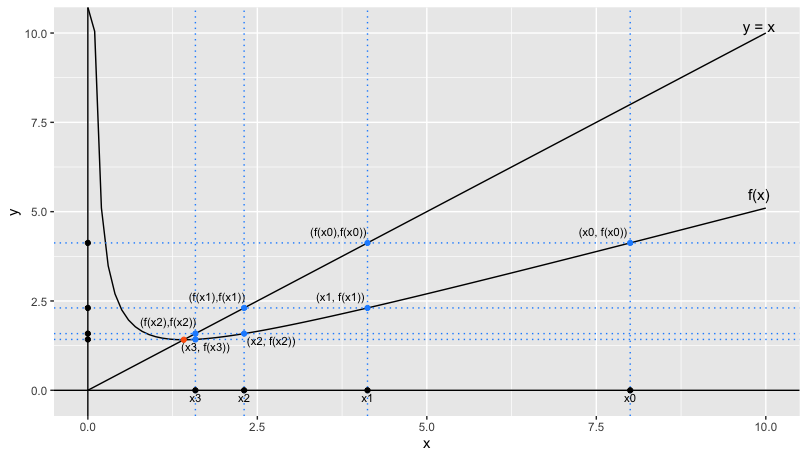
\includegraphics[width=0.8\textwidth]{Successive Approximation Visualization.png}
    \caption{\label{vis:V1}The method of successive substitution}
\end{figure}
Investigating the two curves in Figure \ref{vis:V1}, the method starts by choosing an arbitrary point on $f(x)$, $x_{0}$ on the domain that is defined, and the point has a coordinate $(x_0, f(x_0))$. If $f(x_0) = x_0$ then $(x_0, f(x_0))$ is on the line $y = x$, which means it is a fixed point of $f(x)$. Then, we are done. Otherwise, if $f(x_0) \neq x_0$, then it is not a fixed point. If we make a horizontal line through $(x_0,f(x_0))$, it will intersect $y = x$ at $(f(x_0),f(x_0))$, and then make a vertical line through $(f(x_0),f(x_0))$ which intersects $f(x)$ at $(x_1,f(x_1))$. Since $(f(x_0),f(x_0))$ and $(x_1,f(x_1))$ are on the same vertical line, $x_1 = f(x_0)$. In this way, we create a point that is closer to the fixed point that we want to approach (this conclusion will be justified). Repeating this process, we have $x_2 = f(x_1)$, $\cdots, x_n = f(x_{n-1})$. Hence, we construct a sequence of approximations $\{x_n\}_{n=0}^{\infty}$. If we could prove this sequence converges to some number, then the fixed point of this function exists. In general, the key idea we used to iterate is the following equation (\ref{eqn:ss}).

\begin{equation} \label{eqn:ss}
    x_{n+1} = f(x_{n})
\end{equation}

\end{definition}

\paragraph{  }

With the help of the method of successive substitution, the following theorem could be introduced.

\begin{theorem}[\textbf{Banach Fixed Point Theorem}]\cite{r_kent_nagle_fundamentals_2011}\label{thm:BFPT}
Suppose $g$ is a differentiable function on the closed interval $I$ and $g(x)$ lies in $I$ for all $x$ in $I$. If there exists a constant $K$ such that $\lvert g'(x) \rvert \leq K < 1$ for all $x$ in $I$, then the equation $x = g(x)$ has a unique solution in $I$. Moreover, the sequence of successive approximations defined by 
\begin{equation}\label{eqn:BFPT_sa}
    x_{n+1} = g(x_n), \; n = 0, 1, 2, \cdots
\end{equation}
converges to this solution for any choice of the starting value $x_0$ in $I$.
\end{theorem}

\begin{proof}
    \cite{r_kent_nagle_fundamentals_2011}$(1)$ NTS: $\{x_n\}_{n = 1}^{\infty}$ is well defined. \; We will show this by induction. Base case: By hypothesis, we know that $x_0 \in I$. Then, $x_1 = g(x_0) \in I$ since $g(x)$ lies in $I$ for all $x$ in $I$. Inductive hypothesis: Suppose $x_k \in I$, it suffices to show $x_{k+1} \in I$. Inductive step: $x_{k+1} = g(x_k) \in I$, since $g(x)$ is well-defined in $I$. Then by induction for all $n \in \mathbb{N}$ $\{x_n\}_{n = 1}^{\infty}$ is well-defined.
    
    $(2)$ NTS: $\{x_n\}_{n = 1}^{\infty}$ converges to an element in $I$. \; Let $x_m = S_m = x_0 + (x_1 - x_0) + (x_2 - x_1) + \cdots + (x_m - x_{m-1})$. In order to show $\{x_n\}_{n = 1}^{\infty}$ converges, it suffices to show the partial sum $\{S_n\}_{n = 1}^{\infty}$ converges. We will show that this partial sum sequence converges using the comparison test and the absolute convergence theorem. First, by the mean value theorem, let $p$ and $q$ be two numbers in $I$, then $\exists r \in (p,q) \in I$ such that
    \begin{equation}\label{eqn:MVT}
        g(p) - g(q) = g'(r)(p - q)
    \end{equation}
    Then, since we know 
    \begin{equation}\label{eqn:derivativeBdd}
        \lvert g'(r) \rvert \leq K < 1 \;\;\; \forall r \in I
    \end{equation}
    By assumption, after multiplying $\lvert p - q \rvert$ on both sides of equation (\ref{eqn:derivativeBdd}), we obtain 
    \begin{equation}\label{eqn:a}
        \lvert g'(r)(p-q) \rvert \leq K \lvert p - q \rvert \;\;\; (K < 1)
    \end{equation}
    Then, by substituting equation (\ref{eqn:MVT}) into the equation (\ref{eqn:a}), we have 
    \begin{equation}\label{eqn:bddLink}
        \lvert g(p) - g(q) \rvert \leq K \lvert p - q \rvert
    \end{equation}
    We will show that the sequence $\{S_n\}_{n = 1}^{\infty}$ converges absolutely by proving that each increment in the partial sum is bounded. In other words, we will show $\lvert x_{m+1} - x_{m}\rvert$ is bounded by induction. Base case: Notice, equation (\ref{eqn:bddLink}) applies for all $p$ and $q$ in I. Then, in particular, $\lvert x_2 - x_1 \rvert = \lvert g(x_1) - g(x_0) \rvert \leq K \lvert x_1 - x_0 \rvert$. Hence $\lvert x_2 - x_1 \rvert$ is bounded. Inductive hypothesis: Suppose $\lvert x_{l} - x_{l-1} \rvert$ is bounded by $K^{l-1} \rvert x_1 - x_0 \rvert$; i.e. $\lvert x_{l} - x_{l-1} \rvert \leq K^{l-1} \rvert x_1 - x_0 \rvert$. Inductive step: It remains to show $\lvert x_{l+1} - x_{l} \rvert \leq K^{l} \rvert x_1 - x_0 \rvert$. Indeed, since $\rvert x_{l + 1} - x_l \rvert = \lvert g(x_l) - g(x_{l-1}) \rvert$, then by the equation (\ref{eqn:bddLink}) and the inductive hypothesis, we have
    \begin{equation}
        \rvert x_{l + 1} - x_l \rvert = \lvert g(x_l) - g(x_{l-1}) \rvert \leq K \lvert x_l - x_{l-1}\rvert \leq K \cdot K^{l-1} \rvert x_1 - x_0 \rvert
    \end{equation}
    Hence, we have $\lvert x_{l+1} - x_l \rvert \leq K^l \lvert x_1 - x_0 \rvert \; (K < 1)$. Thus, by induction, we proved that $\lvert x_{m+1} - x_m \rvert \leq K^m \lvert x_1 - x_0 \rvert \; \forall m \in \mathbb{N} \; (K < 1)$. Then 
    \begin{equation}\label{eqn:comparison}
        \sum_{n = 0}^{\infty}{\lvert x_{n+1} - x_n \rvert} \leq \sum_{n = 0}^{\infty}{K^n\lvert x_1 - x_0 \rvert} = \lvert x_1 - x_0 \rvert \sum_{n = 0}^{\infty}{K^n} \; (K < 1)
    \end{equation}
    Thus, since the sequence $\lvert x_1 - x_0 \rvert \sum_{n = 0}^{\infty}{K^n}$ converges to $\lvert x_1 - x_0 \rvert \cdot \tfrac{1}{1-K}$ (notice, $\sum_{n = 0}^{\infty}{K^n}$ is a geometric series with $K < 1$). Then, by the comparison test, we know $\sum_{n = 0}^{\infty}{\lvert x_{n+1} - x_n \rvert}$ converges. Finally, by absolute convergence theorem, we know $\sum_{n = 0}^{\infty}{x_{n+1} - x_n}$ converges, therefore $\{S_n\}_{n = 1}^{\infty} = \{x_0 + \sum_{n = 0}^{\infty}{x_{n+1} - x_n}\}_{n = 1}^{\infty}$ converges. Hence $\{x_n\}_{n = 1}^{\infty}$ converges. Let $x^{*} := \lim_{n \to \infty}{x_n}$, then $x^{*} \in I$, since $I$ is closed.
    
    $(3)$ NTS: $x^{*}$ is a fixed point of function $g(x)$. \; Since $g(x)$ is continuous, then
    \begin{equation}
        x^{*} = \lim_{n\to \infty}{x_{n+1}} = \lim_{n \to \infty}{g(x_n)} = g(\lim_{x \to \infty}{x_n}) = g(x^{*})
    \end{equation}
    Thus, $x^{*}$ is a fixed point of $g(x)$.
    
    $(4)$ NTS: the fixed point $x^{*}$ is unique in $I$. \; We will show this by contradiction. Suppose by contradiction that there is another fixed point $y$ that is different from $x^{*}$, i.e. $y = g(y)$. Then, from equation (\ref{eqn:bddLink}), we have
    \begin{equation}
        \lvert x^{*} - y \rvert = \lvert g(x^{*}) - g(y) \rvert \leq K \lvert x^{*} - y \rvert \Rightarrow (1-K)\lvert x^{*} - y \rvert \leq 0
    \end{equation}
    Since $K < 1$, then $1 - K > 0$, and $\lvert x^{*} - y \rvert$ is non-negative, then $(1-K)\lvert x^{*} - y \rvert$ is non-negative. This forces $(1-K)\lvert x^{*} - y \rvert = 0$, therefore $\lvert x^{*} - y \rvert = 0$. Hence $x^{*} = y$, which is a contradiction, since we assume $x^{*}$ and $y$ distinct. Therefore, $x^{*}$ is unique in $I$.
\end{proof}

\paragraph{   }

The Banach Fixed Point Theorem for functions tells us that when a function $g$ has a unique fixed point in a certain closed interval $I$:
\begin{itemize}
    \item $g$ is differentiable on $I$
    \item the range of $g$ is on $I$, when the domain is on $I$
    \item $\exists K$, such that $\lvert g' \rvert \leq K < 1 \; \forall x \in I$
\end{itemize}

\paragraph{  }

Moreover, the fixed point can be obtained by finding the limit of the sequence of successive approximations of $g$.

\section{Proof of the theorem in $\mathbb{R}$}

\paragraph{  }
In this section, we propose a generalized version of the Banach Fixed Point Theorem by extending it from the version for functions to the version for operators, together with the method of successive substitution for operators. Using these two techniques, we will then prove the existence and uniqueness theorem.

\subsection{Banach Fixed Point Theorem for Operators}

\paragraph{  }

Consider equation (\ref{eqn:operatorEqn}), the solution we want to find is where the input and the image of the operator $F$ meet each other. Recall that this intersection of the input and output is the \textbf{fixed point} of the operator $F$. 

\begin{remark}

We generalize the notion of the fixed point for functions. The \textbf{fixed point of a function} is a point that has the same $x$ and $y$ values, which is the intersection between the function and the line $y = x$. Here we are considering the \textbf{fixed point of an operator} of functions by finding, similarly, a function that maps to itself by applying the operator on it. In other words, it is the intersection of the operator we have and the operator $T(y(x)) = y(x)$

\end{remark}

\paragraph{  }

Extending from the case of functions to operators, we could apply the definition \ref{def:MethodSS} to the operator case. We could follow the same mindset in the previous definition, but the only different thing is that the operator is playing the role of the function in the definition \ref{def:MethodSS}, while the points that we iterated in the previous definition are corresponding to the functions in the new definition of operator.

\begin{definition}[\textbf{The Method of Successive Substituion for Operators}]\label{def:methodSSO}

Similar to the definition \ref{def:MethodSS}, if there is a fixed point $y(x)$ for the operator $F(y(x))$, we could construct a sequence of approximations of functions $\{y_n(x)\}_{n=0}^{\infty}$ that converges to the fixed point of the operator. We describe this recursive procedure using an equation similar to equation (\ref{eqn:ss}):

\begin{equation}\label{eqn:sso}
    y_{n+1}(x) = F(y_n(x))
\end{equation}

Equation (\ref{eqn:sso}) is also called as the \textbf{Picard's Iterations}. The following is an example of how the Picard's Iterations can be applied to an initial value problem.

\begin{example}\label{exm:Picard}
    Compute the Picard iterations for the initial value problem
    \begin{equation}
        y'(t) = y(t)^2 + t
    \end{equation}
    starting with $y_0(x) = 1$
\end{example}
    By defining an operator $\phi$ which maps $y(t)$ to $1 + \int_{0}^{t}{(y_0(x))^2 + x \,dx}$. This I.V.P. is equivalent to 
    \begin{equation}
        y(t) = \phi(y(t)) = 1 + \int_{0}^{t}{y_0(x)^2 + x\,dx}
    \end{equation}
    Computing the Picard iteration via (\ref{eqn:successive}) we find
    \begin{align}
        y_1(t) &= \phi(y_0(t)) = 1 + \int_{0}^{t}{(y(x)^2+x)\,dx} = 1 + \int_{0}^{t}{1^2\,dx} = 1 + t\\
        y_2(t) &= \phi(y_1(t)) = 1 + \int_{0}^{t}{((1+x)^2+x)\,dx} = 1 + \frac{(t+1)^3}{3} + \frac{t^2}{2}\\
        y_3(t) &= \phi(y_2(t)) = 1 + \int_{0}^{t}{((1 + \frac{(x+1)^3}{3} + \frac{x^2}{2})^2+x)\,dx}\\
        &= 1+\frac{4t^7+42t^6+147t^5+245t^4+420t^3+462t^2+448t}{252}\\
        &\cdots 
    \end{align}
\qedwhite
\end{definition}

\paragraph{  }

Notice that in the argument and the proof of the Banach Fixed Point Theorem for functions, we let the sequence created by successive substitutions converge to a unique solution to the original ordinary differential equation. However, instead of having a sequence of numbers, in the operator case, the Picard's Iterations give us a sequence of function. This makes the definition of convergence of a sequence of numbers not sufficient in this case. Hence, we introduce the uniform convergence and the function norm in $\mathbb{R}$ as below to define how a sequence of functions converges uniformly to a function.

\begin{remark}[\textbf{function norm in $\mathbb{R}$}]
    We define a function norm of a function with closed domain $D$ in $\mathbb{R}$ to be:
    \begin{equation}
        \lvert\lvert g(x) - h(x) \rvert\rvert_{D} = max_{x\in D}{\lvert g(x) - h(x)\rvert}
    \end{equation}
\end{remark}

\begin{definition}[\textbf{uniform convergence}]\label{def:uniConv}

A sequence of function $\{y_n(x)\}_{n = 0}^{\infty}$ defined on $C[a,b] \in \mathbb{R}$ \textbf{converges uniformly} to $y(x)$ if and only if $\forall \epsilon > 0, \exists N(\epsilon) \in \mathbb{N}$, such that $\forall n > N, {\lvert\lvert(y_n(x) - y(x)\rvert\rvert} < \epsilon$. i.e. 

\begin{equation}
    \lim_{n \to \infty}{\lvert\lvert y_n(x) - y(x) \rvert\rvert_{[a,b]}} = \lim_{n \to \infty}{max_{[a,b]}{\lvert y_n(x)-y(x)\rvert}} = 0
\end{equation}
Denoted as $y_n(x) \xrightarrow{unif} y(x)$.
\end{definition}

\paragraph{  }

Using this definition, a stronger version of Banach Fixed Point Theorem (also called Contraction Mapping theorem) will be defined as the following:

\begin{theorem}[\textbf{Banach Fixed Point Theorem for Operators}]\cite{r_kent_nagle_fundamentals_2011}\label{thm:BFPTO}
    Let $S$ denote the set of continuous functions on $[a,b]$; i.e.
    \begin{equation}
        S = \{y\in C[a,b]:\lvert\lvert y - y_0\rvert\rvert_{[a,b]} \leq \alpha\}
    \end{equation}
    for some $a, b, \alpha\in \mathbb{R}$. Suppose $T$ is an operator mapping S into $S$ and that $T$ is a \textbf{contraction} on $S$, which means that there exist a constant $K$, $0\leq K < 1$, such that 
\begin{equation}\label{eqn:contractionO}
    \lvert\lvert T(w) - T(z) \rvert\rvert_{[a,b]} \leq K\lvert\lvert w - z \rvert\rvert_{[a,b]}\; \forall w,z \in S
\end{equation}
Then the equation $y = T(y)$ has a unique solution in $S$. Moreover, the sequence of successive approximations given by
\begin{equation}\label{eqn:ssoex}
    y_{n+1} = T(y_n), \; \; \; n = 0, 1, 2, \cdots,
\end{equation}
converges uniformly to this solution for any choice of the starting function $y_0$ in $S$.
\end{theorem}

\begin{proof}
    \cite{r_kent_nagle_fundamentals_2011}$(1)$ NTS: $\{y_n\}_{n = 1}^{\infty}$ is well defined. \; We will show this by induction. By hypothesis, we know that $y_0 \in S$. Then, $y_1 = T(y_0) \in S$ since $T(y)$ lies in $S$ for all $y$ in $S$. Then by induction for all $n \in \mathbb{N}$, $y_n = T(y_{n-1}) \in S$, so that $\{x_n\}_{n = 1}^{\infty}$ is well-defined.
    
    $(2)$ NTS: $\{y_n\}_{n = 1}^{\infty}$ converges to an element in $S$. \; Let $y_m = S_m = y_0 + \sum_{n = 0}^{m}(y_{n+1} - y_n)$. To show $\{y_n\}_{n = 1}^{\infty}$ converges, it suffices to show the partial sum $\{S_n\}_{n = 1}^{\infty}$ converges. We will show that this partial sum sequence converges using the Weierstrass M-test. First, each increment in the partial sum can be proved to be bounded using the contraction assumption by induction. In other words, $\lvert\lvert y_{m+1} - y_{m}\rvert\rvert_{[a,b]}$ is bounded by induction. Notice, equation (\ref{eqn:contractionO}) applies for all $w$ and $z$ in $S$. In particular, $\lvert\lvert y_2 - y_1 \rvert\rvert_{[a,b]} = \lvert\lvert T(y_1) - T(y_0) \rvert\rvert_{[a,b]} \leq K \lvert\lvert y_1 - y_0 \rvert\rvert_{[a,b]}$. Hence, $\lvert\lvert x_2 - x_1 \rvert\rvert$ is bounded by $K \lvert\lvert y_1 - y_0 \rvert\rvert_{[a,b]}$. By induction,
    \begin{align}
        \lvert\lvert y_{m+1} - y_{m} \rvert\rvert_{[a,b]} &\leq K \lvert\lvert y_m - y_{m-1} \rvert\rvert_{[a,b]}\\
        &\leq K^2 \lvert\lvert y_{m-1} - y_{m-2} \rvert\rvert_{[a,b]}\\
        &\leq \cdots\\
        &\leq K^m\lvert\lvert y_1 - y_0 \rvert\rvert_{[a,b]} \; \forall m \in \mathbb{N} \; (K < 1)
    \end{align}
   Then because we define $\lvert\lvert * \rvert\rvert = max_{[a,b]}\lvert * \rvert \in \mathbb{R}$,
    \begin{equation}\label{eqn:comparison2}
        \sum_{n = 0}^{\infty}{\lvert\lvert y_{n+1} - y_n \rvert\rvert_{[a,b]}} \leq \sum_{n = 0}^{\infty}{K^n\lvert\lvert y_1 - y_0 \rvert\rvert_{[a,b]}} = \lvert\lvert y_1 - y_0 \rvert\rvert_{[a,b]} \sum_{n = 0}^{\infty}{K^n} \; (K < 1)
    \end{equation}
    Thus, the sequence $\lvert\lvert y_1 - y_0 \rvert\rvert_{[a,b]} \sum_{n = 0}^{\infty}{K^n} = \lvert\lvert y_1 - y_0 \rvert\rvert_{[a,b]} \cdot \tfrac{1}{1-K}$ (notice, $\sum_{n = 0}^{\infty}{K^n}$ is a geometric series with $K < 1$). Then, by the Weierstrass M-test, we know $\sum_{n = 0}^{\infty}{y_{n+1} - y_n}$ converges uniformly on $C[a,b]$. Hence $\{y_n\}_{n = 1}^{\infty}$ converges uniformly. Let $y^{*} := \lim_{n \to \infty}{y_n}$, then since $y^{*} \in C[a,b]$, $y^{*} \in S$.
    
    $(3)$ NTS: $y^{*}$ is a fixed point of function $T(y)$. \; Let $\epsilon > 0$, $\exists N \in \mathbb{N}$, such that $\forall n > N, \lvert\lvert y_n - y^{*} \rvert\rvert_{[a,b]} < \tfrac{\epsilon}{K}$ because $y_n \xrightarrow{unif} y^{*}$. We will show $\forall n > N, \lvert\lvert T(y_n) - T(y^{*}) \rvert\rvert_{[a,b]} < \epsilon$. Indeed, using the contraction map,
    \begin{equation}
        \lvert\lvert T(y_n) - T(y^{*}) \rvert\rvert_{[a,b]} \leq K \lvert\lvert y_n - y^{*} \rvert\rvert_{[a,b]} < \epsilon
    \end{equation}
    Hence $T(y_n) \xrightarrow{unif} T(y^{*})$. Also, we know $T(y_n) = y_{n+1} \xrightarrow{unif} y^{*}$. Then, since the limit is unique, $T(y^{*}) = y^{*}$. Thus, $y^{*}$ is a fixed point of $T(y)$.
    
    $(4)$ NTS: the fixed point $y^{*}$ is unique in $S$. \; We will show this by contradiction. Suppose by contradiction that there is another fixed point $z$ that is different from $y^{*}$, i.e. $z = T(z)$. Then, from equation (\ref{eqn:contractionO}), we have
    \begin{equation}
        \lvert\lvert y^{*} - z \rvert\rvert_{[a,b]} =\lvert\lvert T(y^{*}) - T(z) \rvert\rvert_{[a,b]} \leq K \lvert\lvert y^{*} - z \rvert\rvert_{[a,b]} \Rightarrow (1-K)\lvert\lvert y^{*} - z \rvert\rvert_{[a,b]} \leq 0
    \end{equation}
    Since $K < 1$, then $1 - K > 0$, and $\lvert\lvert y^{*} - z \rvert\rvert_{[a,b]}$ is non-negative, then $(1-K)\lvert\lvert y^{*} - z \rvert\rvert_{[a,b]}$ is non-negative. This forces $(1-K)\lvert\lvert y^{*} - z \rvert\rvert_{[a,b]} = 0$, therefore $\lvert\lvert y^{*} - z\rvert\rvert_{[a,b]} = 0$. Hence $y^{*} = z$, which is a contradiction, since we assume $y^{*}$ and $z$ distinct. Therefore, $y^{*}$ is unique in $S$.
\end{proof}

\paragraph{   }

The Banach Fixed Point Theorem for operators tells us that when an operator $T$ has a unique fixed point in a certain closed interval $I$:
\begin{itemize}
    \item the range of $T$ is in its domain ($S = \{y\in C[a,b]:\lvert\lvert y - y_0\rvert\rvert_{[a,b]} \leq \alpha\}$)
    \item $T$ is a contraction mapping
\end{itemize}

\subsection{Applying Theorem \ref{thm:BFPTO} to prove Theorem \ref{thm:EUT}}\label{sec:3.5}

\paragraph{  }

Continuing our derivation in the section \ref{sec:3.2}, when we want to find a unique solution to the problem (\ref{eqn:ode}), we are actually solving a problem (\ref{eqn:operatorEqn}) with a defined operator $F(y(t)) = y_0 + \int_{0}^{t}{f(s,y(s))} \,ds$. In this way, we want to find a unique fixed point of the operator $F$ in a specific interval $I = [-h, h]$. 

\begin{proof}
    \cite{r_kent_nagle_fundamentals_2011}We will use the Theorem \ref{thm:BFPTO} (Banach Fixed Point Theorem for Operators) to prove that the equation $y = F(y)$ has a unique solution in an interval $I = [-h, h]$. 

    First, we choose positive $h_1, \alpha$ such that 
    \begin{equation}
        R_1 = \{(t,y)\lvert \lvert t \rvert \leq h_1, \lvert y - y_0 \rvert \leq \alpha\} \subset R
    \end{equation}
    Since $f$ and $\tfrac{\partial f}{\partial y}$ are both continuous in $R$, they are continuous in $R_1$. Then $\forall (t,y) \in R_1$, we know that $\exists M, L \in \mathbb{R}$ such that
    \begin{equation}\label{eqn:bddAssumption}
        \lvert\lvert f(t,y) \rvert\rvert_{R_1} \leq M \text{, and }\left\lvert\left\lvert \dfrac{\partial f(t,y)}{\partial y} \right\rvert\right\rvert_{R_1} \leq L
    \end{equation}
    Because the continuous image of a connected set (an interval) is connected (an interval), the image is bounded. Let $S = \{g \in C(I) \lvert \lvert \lvert g - y_0\rvert\rvert_{I} \leq \alpha\}$. Choose $0 < h < min\{h_1, \tfrac{\alpha}{M}, \tfrac{1}{L}\}$, we will show that the assumptions of the Theorem \ref{thm:BFPTO} are met; i.e. $F(y)$ is a contraction map mapping $S$ to $S$.
    Let $g(t) \in S$, then $g(t)$ is a continuous function, and $\lvert g(t) - y_0 \rvert \leq \alpha\; \forall x \in I$. Then we will show $F(g) \in S$, i.e. $\lvert\lvert F(g) - y_0 \rvert\rvert_{I} \leq \alpha$. Indeed, first, by the way we choosing $h$, it is obvious that $I \subseteq [-h_1, h_1]$, then $\lvert\lvert f(t,y) \rvert\rvert_{I} \leq M \text{, and }\left\lvert\left\lvert \tfrac{\partial f(t,y)}{\partial y} \right\rvert\right\rvert_{I} \leq L$, then: 
    \begin{align}
        \left\lvert\left\lvert F(g) - y_0 \right\rvert\right\rvert_{I} &= \left\lvert\left\lvert y_0 + \int_{0}^{t}{f(s,g(s))}\,ds - y_0\right\rvert\right\rvert_{I}\\
        &=\left\lvert\left\lvert \int_{0}^{t}{f(s,g(s))}\,ds\right\rvert\right\rvert_{I} \leq \left\lvert\int_{0}^{t}{\lvert\lvert f(s,g(s))\rvert\rvert_{I}}\,ds\right\rvert\\
        &\leq \left\lvert\int_{0}^{t}{M}\,ds\right\rvert = M\left\lvert \int_{0}^{t}{1}\,ds\right\rvert = M\lvert t - 0\rvert\\
        &\leq Mh \leq M\cdot (\tfrac{\alpha}{M}) \leq \alpha
    \end{align}
    Then, we will show that $F$ is a contraction on $S$ by showing that $\forall v < u \in S, \lvert\lvert F(u) - F(v) \rvert\rvert_I \leq \lvert\lvert u - v \rvert\rvert_I$. Indeed, using the mean value theorem for two variables, there exist $v(s) < z(s) < u(s) \; \forall s \in I \subseteq R_1$, such that:
    \begin{align}
        \lvert\lvert F(u) - F(v) \rvert\rvert_I & = \left\lvert\left\lvert \int_{0}^{t}{(f(s,u(s)) - f(s,v(s))) \,ds} \right\rvert\right\rvert_I\\
        & = \left\lvert\left\lvert \int_{0}^{t}\tfrac{\partial f}{\partial y}(s,z(s)){(u(s) - v(s))} \,ds \right\rvert\right\rvert_I\\
        & \leq L\left\lvert\int_{0}^{t}{\lvert\lvert u(s) - v(s) \rvert\rvert_I \,ds}\right\rvert\\
        & \leq L\lvert\lvert u - v \rvert\rvert_{I} \left\lvert \int_{0}^{t}{1}\,ds \right\rvert \leq L\lvert\lvert u - v \rvert\rvert_{I}\lvert t \rvert\\
        & \leq Lh\lvert\lvert u - v \rvert\rvert_{I} \leq L \cdot(\tfrac{1}{L})\lvert\lvert u - v \rvert\rvert = \lvert\lvert u - v \rvert\rvert
    \end{align}
    Hence, we can now apply the Theorem \ref{thm:BFPTO} and claim that there is a unique fixed point $y^{*} \in S$ of $F$. Then, there exists a unique solution to the ordinary differential equation (\ref{eqn:ode}) in $S$ which is continuous in $I$. Moreover, the sequence of successive approximations given by
    \begin{equation}
       y_{n+1} = F(y_n), \; \; \; n = 0, 1, 2, \cdots,
    \end{equation}
    converges uniformly to this unique solution for any choice of the starting function $y_0$ in $R$.
\end{proof}
    
\begin{example}
    Find an interval [-h,h] over which the I.V.P. in the previous example \ref{exm:Picard} is guaranteed to have a unique solution by the Picard Iteration.
\end{example}
We first pick a rectangle R centered at the initial point (0,1). Let $R :=\{(t,y): -2 < t < 2, -1 < y < 3\}$. Notice that both $f:= y^2$ + t and $ \frac{\partial f}{\partial y}$ = 2y are continuous inside.
Next, we choose a closed rectangle contained in R. Let $R_1:=\{(t,y): -1 \leq t \leq 1, 0 \leq y \leq 2\}$. Inside $R_1$ we can easily derive the bounds
\begin{equation}
    \lvert\lvert f(t,y) \rvert\rvert_{R_1} \leq 2^2 + 1 = 5
\end{equation}

and

\begin{equation}
    \left\lvert\left\lvert \frac{\partial f}{\partial y} (t,y) \right\rvert\right\rvert_{R_1} \leq 2*2 = 4
\end{equation}

Thus, the parameters $h_1$, $\alpha$, M, and L in the theorem will be

\begin{equation}
    h_1 = 1, \alpha = 1, M = 5, L = 4
\end{equation}

Thus, the choice $h = min\{ 1, \tfrac{1}{5}, \tfrac{1}{4} \} = \tfrac{1}{5}$ suffices. So, a unique solution is guaranteed to exist for $-0.2 \leq x \leq 0.2$. \qedwhite

\section{The Existence and Uniqueness Theorem in a General Metric Space $(X,d)$}

\subsection{Definition of a metric space}

\paragraph{  }
Before proving the existence and uniqueness theorem in a general metric space, we need to know what properties that general metric space has. Hence, we define the metric space as following.

\begin{definition}[\textbf{Metric Space}]\label{def:matricSpace}

A \textbf{metric space} $(X,d)$ satisfies the below three properties $\forall x,y \in X$ 

\begin{itemize}
    \item $d(x,y) \geq 0$ and $d(x,y) = 0 \Longleftrightarrow x = y$
    \item $d(x,y) = d(y,x)$
    \item $d(x,z) \leq d(x,y) + d(y,z)$
\end{itemize}

Additionally, $d$ is also called as the metric of the metric space $(X,d)$
\end{definition}

\paragraph{  }

In this section, the version of the Existence and Uniqueness Theorem in a metric space requires some special properties of the metric space $(X,d)$. To be more specific, we need the following definition:

\begin{definition}[\textbf{norm induced metric}] \cite{rudin_functional_nodate}
    A norm induced metric $d$ of a metric space $(X,d)$ needs to satisfy the following two properties:
    \begin{itemize}
        \item \textbf{(homogeneous)} $\lvert \lambda \rvert d(x,y) = d(\lambda x, \lambda y) \;\forall \lambda \in \mathbb{R}$
        \item \textbf{(translation-invariant)} $d(x,y) = d(x+z,y+z) \;\forall z \in X$
    \end{itemize}
\end{definition}

\subsection{Metric space version of convergence and Cauchy}

\paragraph{  }

Now, we have the definition of metric space, we still need the properties for convergence. Thus, we refine the definitions of convergence, uniform convergence, and Cauchy sequences in the metric space.

\begin{definition}[\textbf{convergence of a sequence in a norm induced metric space $(X,d)$}]\label{def:ConvMetric}
    A sequence $\{x_n\}_{n=1}^{\infty} \subseteq X$ converges to $x \in X$ if and only if $\forall \epsilon > 0, \exists N(\epsilon) \in \mathbb{N}$, such that $\forall n > N, d(x_n - x) < \epsilon$. i.e. 
    \begin{equation}\label{eqn:ConvMetric}
        \lim_{n \to \infty}{d(x_n - x) = 0} \;\;\; \forall n > N
    \end{equation}
\end{definition}

\begin{definition}[\textbf{uniform convergence in a norm induced metric space $(X,d)$}]\label{def:uniConvMetric}

    A sequence of function $\{y_n(x)\}_{n = 0}^{\infty}$ defined on $D \subseteq X$ converges uniformly on $D$ to $y(x)$ if and only if $\forall \epsilon > 0, \exists N(\epsilon) \in \mathbb{N}$, such that $\forall n > N, d(y_n(x) - y(x)) < \epsilon$. i.e.
        \begin{equation}
            \lim_{n \to \infty}{d(y_n(x) - y(x))} = 0 \;\;\; \forall n > N
        \end{equation}
    Denoted as $y_n(x) \xrightarrow{unif} y(x)$
\end{definition}

\begin{definition}[\textbf{Cauchy Sequences}]\label{def:cauchySeq}

    A sequence $\{x_n\} \subset X$ is called Cauchy if $d(x_n - x_m) \rightarrow 0$ as $m,n \rightarrow \infty$, i.e. if for any $\epsilon < 0$ there is $N = N(\epsilon)$ such that
        \begin{equation}
            \forall m,n > N \Longrightarrow d(x_n - x_m) < \epsilon
        \end{equation}
\end{definition}

To prove the existence and uniqueness theorem in the general metric space, we seek to use the similar ideas to the Banach Fixed Point Theorem as we did in the previous section. We will prove the contraction mapping theorem, which states that a contraction mapping is guaranteed to have a fixed point.

Before proving this theorem, however, we still need the definition of completeness and the definition of contraction.

\begin{definition}[\textbf{Completeness}]\label{def:completeness}

    A subset S of X is said to be complete if every Cauchy sequence $\{x_n\}_{n = 1}^{\infty} \subset S$ converges to a point $x \in S$
\end{definition}

\begin{definition}[\textbf{Contraction}]\label{def:contraction}

    Let $(X,d)$ be a metric space. A mapping $A :X\rightarrow X$ is said a contraction if there exists an $\alpha,\ 0<\alpha<1,$ such that
        \begin{equation}
            d(A(x),A(y)) \leq \alpha d(x,y), \forall x,y \in X
        \end{equation}
\end{definition}

\subsection{Proof of the Theorem in (X,d)}

\paragraph{  }

Now, we are ready to prove the Contraction Mapping theorem using the definitions that we stated so far.

\begin{theorem}[\textbf{Contraction Mapping theorem}]\cite{holmes_chapter_2016}\label{thm:CMT}
    Let $(X,d)$ be a complete metric space, and $A:X\rightarrow X$ be a contraction mapping. Then A has a unique fixed point in X. That is, there is a unique point $x^*\in X$ such that $A(x^*) = x^*$. Furthermore, if $x_0$ is any point in X, and define $x_{n+1} = A(x_n)$, then $x_n \rightarrow x^*$ as $n \rightarrow \infty$.
\end{theorem}

\begin{proof}

    We will show $\{x_n\}$ converges to $x^* \in X$. i.e., $x^*$ is a fixed point. Since $X$ is a complete metric space, it suffices to show that $\{x_n\}_{n = 1}^{\infty}$ is a Cauchy sequence. Now, for $n = 1,2, \cdots$, we apply Definition \ref{def:contraction} repeatedly and obtain the following
        \begin{equation}
            d(x_{n+1},x_n) = d(A(x_n),A(x_{n-1})) \leq \alpha d(x_n,x_{n-1}) \leq \alpha^2 d(x_{n-1},x_{n-2}) \leq \cdots \leq \alpha^n d(x_1,x_0)
        \end{equation}
        
    Let n, m $\in \mathbb{N}$, by triangle inequality, we have
    
        \begin{align}
            d(x_{n+m},x_n) &\leq \sum_{i=1}^{m} d(x_{n+i},x_{n+i-1})\\
            &\leq \sum_{i=1}^{m} \alpha^{n+i-1} d(x_0,x_1)\\
            &\leq \frac{\alpha^n}{1-\alpha}d(x_0,x_1) \rightarrow 0  \ as\ n \rightarrow \infty
        \end{align}
    Thus, $\{x_n\}$ is a Cauchy sequence
    To prove this fixed point $x^{*}$ obtained is unique, we will prove by contradiction. Suppose by contradiction that there exists another fixed point $y$ of $A$, then $y = A(y)$. Hence,
    \begin{equation}
        d(x^{*},y) = d(A(x^{*}),A(y)) \leq \alpha d(x^{*},y) \implies (1-\alpha)d(x^{*},y) \leq 0
    \end{equation}
    Since by definition \ref{def:contraction}, $0 < \alpha < 1$, then $1-\alpha > 0$, and therefore $d(x^{*},y) = 0 \implies x^{*} = y$. Thus, $x^{*}$ is unique in $X$
\end{proof}

Basically a metric space defines a distance between the objects in a field. With the above definitions and theorems stated in a metric space, we can state a general version of Theorem \ref{thm:EUT} within a general metric space $(X,d)$. 

The proof of this theorem is similar to the one we did previously, we will define a mapping and apply the contraction mapping theorem that we have just proved. Then, we will use this result to prove there exists a unique solution to the Initial Value Problem.

\begin{theorem}[\textbf{The Existence and Uniqueness Theorem in $(X,d)$}]\cite{r_kent_nagle_fundamentals_2011}\label{thm:EUTXd}
    Define $(X,d)$ is a complete norm-induced metric space. Let $f$ and $\tfrac{\partial f}{\partial y}$ be continuous in the rectangle $R = \{(t,y)|a < t < b, c < y < d\} \subseteq X$ where $a,b,c,d \in X$ and the rectangle contains the point $(0, y_0) \in R \subseteq X$. Then the initial problem
    \begin{equation}
        \dfrac{\,dy}{\,dt} = f(t,y),\; y(0) = y_0
    \end{equation}
has a unique solution in some interval $I = [-h, h]$, where h is an element in $X$.
\end{theorem}

\begin{proof}
    \cite{r_kent_nagle_fundamentals_2011}First, define a map 
    \begin{align}
        \Phi: \,&X \rightarrow X\\
        &y \mapsto y_0 + \int_{0}^{t}f(s,y(s))\,ds
    \end{align}
    Following the similar argument in the section \ref{sec:3.1}, we could show that the ode problem in the Theorem \ref{thm:EUTXd} have the same solution as $y = \Phi(y)$.
    
    To solve this problem, it suffices to prove there exists a unique fixed point of the map $\Phi$ in $X$. Similar to the Section \ref{sec:3.5}, we will apply Theorem \ref{thm:CMT} (Contraction Mapping Theorem) to Theorem \ref{thm:EUTXd} in the metric space $(X,d)$. We choose positive $h_1, \alpha \in X$ such that 
    \begin{equation}
        R_1 = \{(t,y) \lvert d(t,0) \leq h_1, d(y, y_0) \leq \alpha\} \subset R
    \end{equation}
    Because $f$ and $\tfrac{\partial f}{\partial y}$ are continuous on $X$, they are continuous on $X_1$, and they are bounded in $X_1$; i.e. $\exists M, L \in X$ such that 
    \begin{equation}
        d(f(t,y),0) \leq M \text{, and } d\left(\dfrac{\partial f(t,y)}{\partial y},0\right) \leq L
    \end{equation}
    Let $S := \{g \in C(I)\lvert d(g,y_0) \leq \alpha\}$. Choose $0 < h < min\{h_1, \tfrac{\alpha}{M},\tfrac{1}{L}\}$, we will show that $\Phi(y)$ is a contraction mapping from $S$ to $S$. Let $g(t) \in S$, then $g(t)$ is a continuous function by definition, and $d(g,y_0) \leq \alpha \; \forall x \in I$. Then we will show $\Phi(g) \in S$, i.e. $d(\phi(g),y_0) \leq \alpha$. Indeed,
    \begin{align}
        d(\Phi(g),y_0) &= d\left(y_0+\int_{0}^{t}{f(s,g(s))}\,ds,y_0\right)\\
        &=d\left(\int_{0}^{t}{f(s,g(s))}\,ds,0\right)\\
        &\text{(by the translation-invariant property)}\\
        &\leq \int_{0}^{t}{d\left(f(s,g(s)),0\right)}\,ds\\
        &\leq M \int_{0}^{t}{1}\,ds = M\cdot d(t,0)\\
        &\leq Mh \leq M\cdot (\dfrac{\alpha}{M}) \leq \alpha
    \end{align}
    Then, we will show that $\Phi$ is a contraction on $S$ by showing that $\forall u,v \in S, d(\Phi(u),\Phi(v)) \leq d(u,v)$. Indeed, using the mean value theorem for two variables, there exists $v(s) < z(s) < u(s) \; \forall s \in I \subseteq X_1$, such that:
    \begin{align}
        d(\Phi(u),\Phi(v)) &= d\left(y_0+\int_{0}^{t}{f(s,u(s))}\,ds, y_0+\int_{0}^{t}{f(s,v(s))}\,ds\right)\\
        &= \int_{0}^{t}{d(f(s,u(s)), f(s,v(s)))}\,ds\\
        &\text{(by the translation-invariant property)}\\
        &\leq \int_{0}^{t}{\tfrac{\partial f}{\partial y}(s,z(s))d(u(s),v(s))}\,ds \text{ (by the mean value theorem)}\\
        &\leq \int_{0}^{t}{L \cdot d(u(s),v(s))}\,ds\\
        &= L\cdot d(u,v) \int_{0}^{t}{1}\,ds = L \cdot d(0,t) \cdot d(u,v)\\
        &\leq Lh\cdot d(u,v) \leq L \cdot (\tfrac{1}{L})\cdot d(u,v) = d(u,v)
    \end{align}
    Hence, the assumption for Theorem \ref{thm:CMT} is met, then there exists a unique fixed point $y^{*} \in S$ of $\Phi$. This means that there exists a unique solution to the ordinary differential equation in $S \in X$ which is continuous in $I$. Moreover, the sequence of successive approximations given by
    \begin{equation}
       y_{n+1} = \Phi(y_n), \; \; \; n = 0, 1, 2, \cdots,
    \end{equation}
    converges uniformly to this unique solution for any choice of the starting function $y_0$ in $X$.
\end{proof}

\section{Conclusion}

\paragraph{  }

In order to determine whether an ordinary equation has a solution in a certain interval without solving for explicit formulas, we need help from the Existence and Uniqueness Theorem. In this project, we first proved the Theorem in $\mathbb{R}$ using the Banach Fixed Point Theorem for operators, and then obtained the approximation for the unique solution by the Picard Iterations. Second, we extend our claim into a general metric space $(X,d)$ with a norm induced metric $d$. We used the successive substitution again to approximate the unique solution in the general metric space.

\newpage
\bibliographystyle{alpha}
\bibliography{sources}

\end{document}